\documentclass{article}
\usepackage{csvsimple}
\usepackage{amsmath}
\usepackage{amssymb}
\usepackage{graphicx}
\usepackage{hyperref}
\usepackage{wrapfig}

\begin{document}

%insert your content here..

\section{Student content}

\subsection{Doug Healy}

I am starting my second year in work towards my PhD in Engineering Security, studying under Dr. Bloom. I received my Masters in Information Security Policy and Management (MSISPM) from Carnegie Mellon in 2013, and my BS in Electrical Engineering Technology back in 2003 from the Rochester Institute of Technology (RIT). 

I am a avid and active supporter of Scouts BSA, volunteering much of my time in support of the program, both at the Scout (11 to 18 years old) and Cub Scout (5-11 years old) levels. Being an Eagle Scout myself, I highly believe in the values and qualities it instills in our young men and women and work very hard to make the programs successful and FUN!  

For this course, I hope to become more efficient in my research. I have spent many, many hours over the summer pouring over search results from both Google Scholar and the UCCS Library. I want to learn how to hone search results, use the correct resources, to efficiently find what I am actually looking for, not what some search engine "thinks" I am looking for. This will also require me to refine how I choose my search terms.  

Secondly, I want to learn how to effectively learn to use my time in reading a scholarly document. I am not a good "skimmer" of documents or books; never have been. I want to learn how to do this more effectively and to make sure I am not missing anything. I always think I am missing important things on the page, and I want to ensure that through my skimming, I am not.   

%\subsection{My Picture: }
\begin{figure}[h]
    \centering
    \includegraphics[scale=.095]{Healy.jpg}
    \caption{Doug Healy at Philmont Scout Ranch, Cimarron NM}
 \end{figure}

\subsection{Will Wesley}
\subsubsection{Introduction}
In authoring \emph{Go To Statement Considered Harmful}
% doing as a footnote, because I couldn't think of a better way to cite in this shared thing.
% yes, I briefly considered adding a bib and whatnot, but didn't want to make life hard for other contributors.
\footnote{E. Dijkstra, “Letters to the editor: go to statement considered harmful,” Commun. ACM, vol. 11, pp. 147–148, 1968.}
Dijkstra is credited for giving birth to structured programming by some
\footnote{E. N. Yourdon, Ed., Classics in Software Engineering: Go to Statement Considered Harmful.
USA: Yourdon Press, p. 27–33.}.
But, I think he set a precedent that many overlook.
There are certain things that one \emph{can} do when creating software, but for the sake of the humans involved, one \emph{shouldn't}.

\begin{wrapfigure}[13]{l}{0.3\linewidth}
  \includegraphics[width=\linewidth]{Wesley}
  \caption{Will}
  \label{fig:will}
\end{wrapfigure}
Dijkstra said that by restricting how we enter blocks of code, we get some guarantees about what to expect of the system state inside those blocks.
We use typing systems to give us some guarantees about our usage of data in a program, even though data coercion and ``duck typing'' have certain advantages.
Functional programming gives us guarantees about the behavior of functions, while restricting our ability to assign values.

I suspect that there is another set of restrictions, or perhaps disciplines, that can be shown to also make software better with respect to the humans who have to maintain it.

My goals in this course are to develop better skills in researching and find a meaningful question to answer that relates to testing software in a disciplined manner, as I suspect doing so can be shown to yield superior software.

I am currently studying for a Master's of Computer Science, which I expect to complete this semester.
I will be starting my PhD research in the spring.
This fall, I will also be testing for my Second Degree Black Belt in Taekwondo.

\subsubsection{Sneaky added requirement}
\url{https://github.com/stryker-mutator/stryker-js} is a mutation testing tool for JavaScript.
Mutation testing is kind of a way to test the test suite.
If you have a test suite that has high code coverage, but asserts very little about the behavior of the code, how do you know it does what you want?
The idea of mutation testing is to present the test suite with broken, mutated versions of your production code to see if it can detect the change.
If it can't, you can be sure the test suite is insufficient.

An interesting thing to note is that research shows that software test suites with better mutation scores (detect lots of mutations) correspond to fewer bugs found in the production code\footnote{J. H. Andrews, L. C. Briand, and Y. Labiche, ``Is mutation an appropriate tool for testing experiments?,'' in Proceedings of the 27th International Conference on Software Engineering, ICSE ’05, (New York, NY, USA), p. 402–411, Association for Computing Machinery, 2005.}.
Further, I believe that the practice of TDD leads to better mutation scores.

\subsubsection{Q \& A}
\begin{enumerate}
    \item AN: How hard was it for you to ramp up on Computer Science?

    Well, I've been playing with computers since I was eight when my mom bought me a TRS-80.
    So, maybe not hard, just a long time.
    \item
\end{enumerate}
\subsection{Section 1 - About Me}

From Week 1, the definition of research is “a combination of investigation.” I hope to learn everything that I can about “investigation” and common tools in accomplishing that. I believe one of my skills, like reading research papers more effectively, can be further improved. More importantly, I bring in the mentality of being curious and grit. Being curious allows me to explore and wonder while grit allows me to dig deep into certain topics that would help with my research. My mission and goal for this CS6000 course is to get the perspective in understanding elements of good research that sparks my interest and passion, while making an impact on society. I am currently in my first semester of the PhD security program here at University of Colorado, Colorado Springs. With the nature of the program, I would also like to learn on how to effectively present my ideas and convey my research to the languages of different audiences. My research topic will be close to Blockchain technology with its performances and implementation. 

\begin{center}

\includegraphics[scale=0.45]{kl.png}
\end{center}

Some of my recent interests besides information technology would be aviation and endurance sports. I have a little more than 100 hours in a Cessna 172M model and I will be running a 50k trail run this coming October.

\subsection{Section 2 - Git Repo}

\subsubsection{Git Repo - Research}
I found this Git Repo to be useful in learning more about Blockchain. This git repo covers topic from basics of blockchain all the way to development and implementation of blockchain.
\url{https://github.com/yjjnls/awesome-blockchain}


\subsubsection{Questions and Answer} 
You may include your question here:

\begin{enumerate}
    \item WW: Do you have anything interesting to share from your research into Blockchain thus far?
    \item DH: Where are you doing your trail run, and is it with an organized team or an individual effort?
\end{enumerate}

\subsection{Andrew Nielsen}

I'm working towards getting my Masters degree in Cybersecurity. My goal for this course is to be able to prepare for my PhD down the road and be able to apply the research knowledge I gain from this class herein. I'm hoping to learn how to read efficiently and quickly navigate through research documents. I'm looking to be able to understand how to research and how to narrow down a topic that will help in the future. I'm studying cybersecurity in the master's program. 

The research area that I have been working on is ransomware with fuzzy techniques in geo-spatial systems. Part of it has been in understanding ransomware, fuzzing, and identifying gaps in geo-spatial research extending past the earth's atmosphere.

Some code that I found on GitHub that deals with ransomware was found \href{https://github.com/mauri870/ransomware.git}{here}. This code actually simulates how ransomware behaves and encrypts all the files on a machine and stores the encryption key on a remote server so the user is not able to decrypt their files. I did not have to deal with any merge conflicts when updating files and committing them back to the repository.


A picture of myself can be seen below:

\begin{figure}[htp]\centering

\includegraphics[width=.3\textwidth]{Andrew Professional picture.jpg}
\caption{Andrew Nielsen's Picture}
\label{fig:Andrew Professional picture}
\end{figure}

\subsubsection{QA}

\begin{enumerate}
    \item WW: Where did you do your undergrad?

	AN: I did my undergrad at Weber State University in Accounting and Information Systems and Technology. 

    \item DH: How soon are you looking to start your PhD? Directly after your Master's?

	AN: The more I think about it the more that I want to wait as the work i'm currently doing doesn't line up to much with research. It may not be until kids are out of the house. haha
\end{enumerate}


\subsection{Logan Montgomery}
My immediate tangible goal is to get use to being retired (27 July).  Next, I want to complete my second M.S. in Computer Science.  Following my second M.S., I want to pursue a PhD in Computer Science, gain meaningful employment as a University Professor, and continue research in various domains impacted by or dependent on computer science.  Intangibly, “I am a lifelong learner.”  I do not have an objective or completion date for my journey through curiosity, education, and research.  My goal is simple, “breath, engage in life, learn, and influence change where possible.”

\begin{figure}[ht]
	\centering
    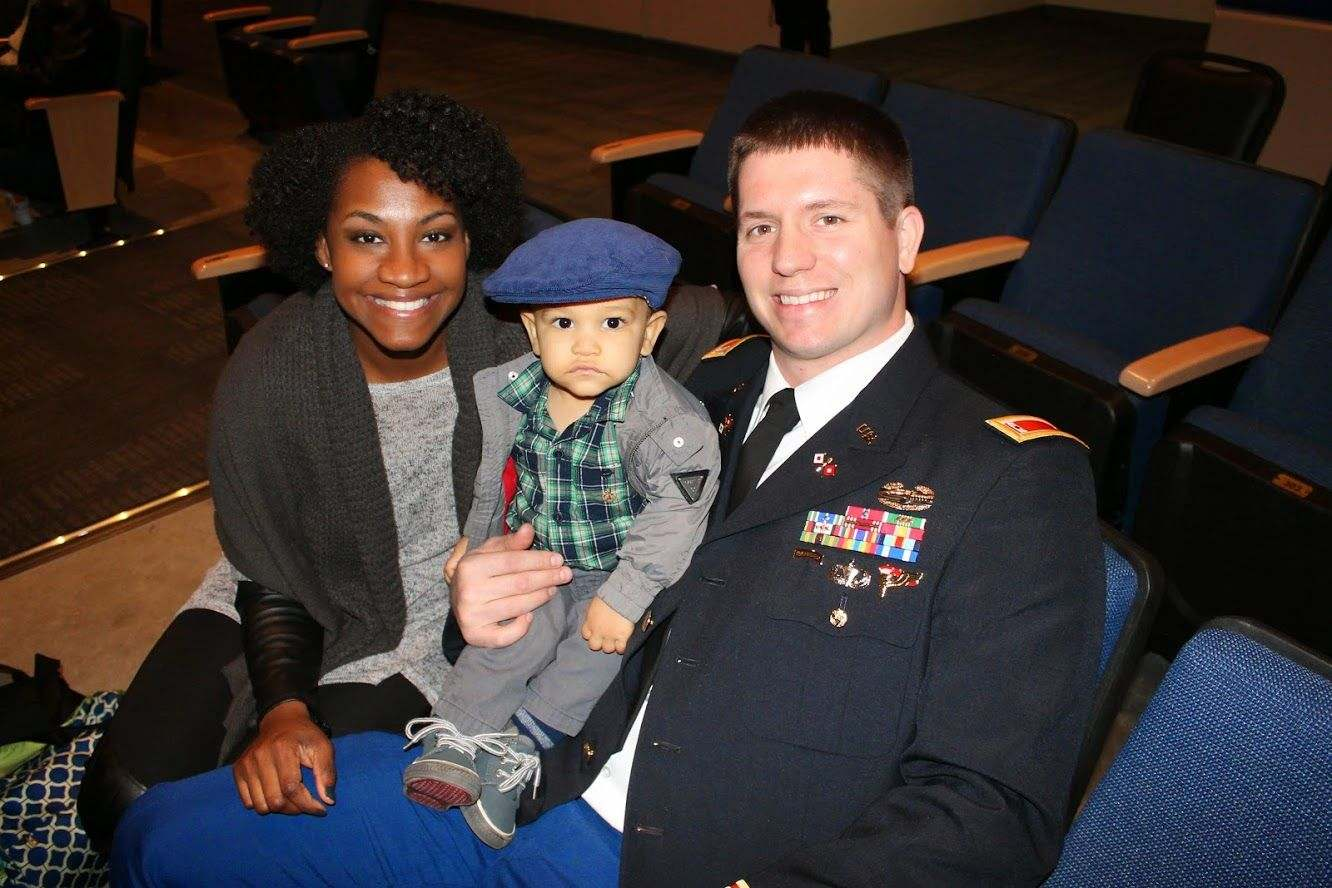
\includegraphics[width=3in]{myimage}
    \caption{My Family and I}
    \label{fig:My Family and I}
\end{figure}

\subsection{Related GIT - Covert Channel Through TCP Checksums Using SCAPY}
I chose a random covert channel git repo.  I don't have a research area officially, but I play around with network security and data exfiltration techniques regularly.  So, I though I'd share a pretty straight forward method of transferring data by crafting TCP checksums using SCAPY.   

\url{https://github.com/mtarsel/Covert-Channel}

\subsubsection{QA}
\begin{enumerate}

	\item RR: I thought your choice of git repo was interesting, I have not played with SCAPY before. Do you think Covert Channel communications could become one of your research topics in the future?
	
        \item KA: Have you design small system such as chat using socket programming and Is there any educational version for Wireshark?

\end{enumerate}

\subsection{Ryan Rabinowitz}

I am currently enrolled in the Cybersecurity Master of Engineering program at the University of Colorado, Colorado Springs.
Some of my personal interests are 3D Printing (FDM only), Photography, Bowling, and flying my quadrocopter, I also have a small tabby cat named Morty. 
My research areas of interest are Computer Vision, Blockchain Systems, and Steganographic Systems, although I am interested in many projects involving cryptography that lie outside these topics. 

In CS 6000 I hope to start building on a wealth of skills required to create and publish meaningful research.
Namely, I would like to become more comfortable with LaTex and become more effective at skimming papers quickly. 
Co-authoring my first paper over the summer has gotten me familiar with overleaf and LaTex, but also revealed there is a long road ahead to mastery. 
As far as effective skimming of papers goes, I have read with care my entire life so skimming is somewhat counter-intuitive. 
From my understanding of CS 6000, I will be forced to confront this, which will be (hopefully) be a good thing.

A Git repo related to my research is RBF-Softmax \url{https://github.com/2han9x1a0release/RBF-Softmax.git}, a pytorch implementation of several common computer vision networks with Radial Basis Function-Softmax instead of a normal linear classifier head. 
The goal of RBF softmax is to shape the feature space of the network such that features of images within a given class are tightly clustered and class centers are spread apart from one another.
\begin{figure}[h]

\includegraphics[width=8cm]{Rabinowitz_Headshot.jpg}
\end{figure}

\item KA: I am wondering what is the improvement of deep learning models when you use RBF-Softmax?

\documentclass{article}
\usepackage[utf8]{inputenc}
\usepackage{graphicx}
\usepackage{biblatex}
\usepackage{blindtext}
\usepackage[section]{placeins}
\usepackage{amsmath}
\addbibresource{citing.bib}
\graphicspath{ {./image/} }
\title{Git Assignment}
\author{Moses Smith Guddah}
\date{September 21 2021}

\subsection*{Section I:  Introduction }

I am a Ph.D. student and Graduate Teaching Assistant with the College of Engineering and Applied Science, University of Colorado, Colorado Springs (UCCS). My research interests focus on High Performance Computing systems with specific focus on memory management for Load balancing systems. 

Even though I have had some research experience in Business Management, this course syllabus presents aspects of Computer Science research broadly and very differently from what I have previously done in Business. It is my hope this course enables me understand the knowledge required for being an excellent Computer Science researcher. Further, it is my desire to use the knowledge gained through this course for publishing papers, which is a cardinal part of my Ph.D. program.  

I have worked in the telecommunication industry over the last fifteen years as a Network Deployment Engineer, Intelligent Network Engineer, Network Administrator and a Project Administrator. Those fifteen years allowed my teams deploy cutting-edge technologies in developing country across some regions of Africa that improved mobile communication.

On a personal level, my broader interests lie in understanding how cultural dynamics and micro politics within scientific communities, and public policies impact quality scientific research. There is a schism between science, and politics and culture that has confronted society. Though much has been done to narrow that divide, there is definitely more of understand and influence, so that policy- makers can support scientific communities for significant and impacting research. I am an ardent Tennis player and a  lover of running  trails.

I am married to an intelligent, beautiful, resourceful lady, Jemu Zarzar- Guddah and we have a two-year-old daughter.

\begin{figure}[hbt!]
    \centering
    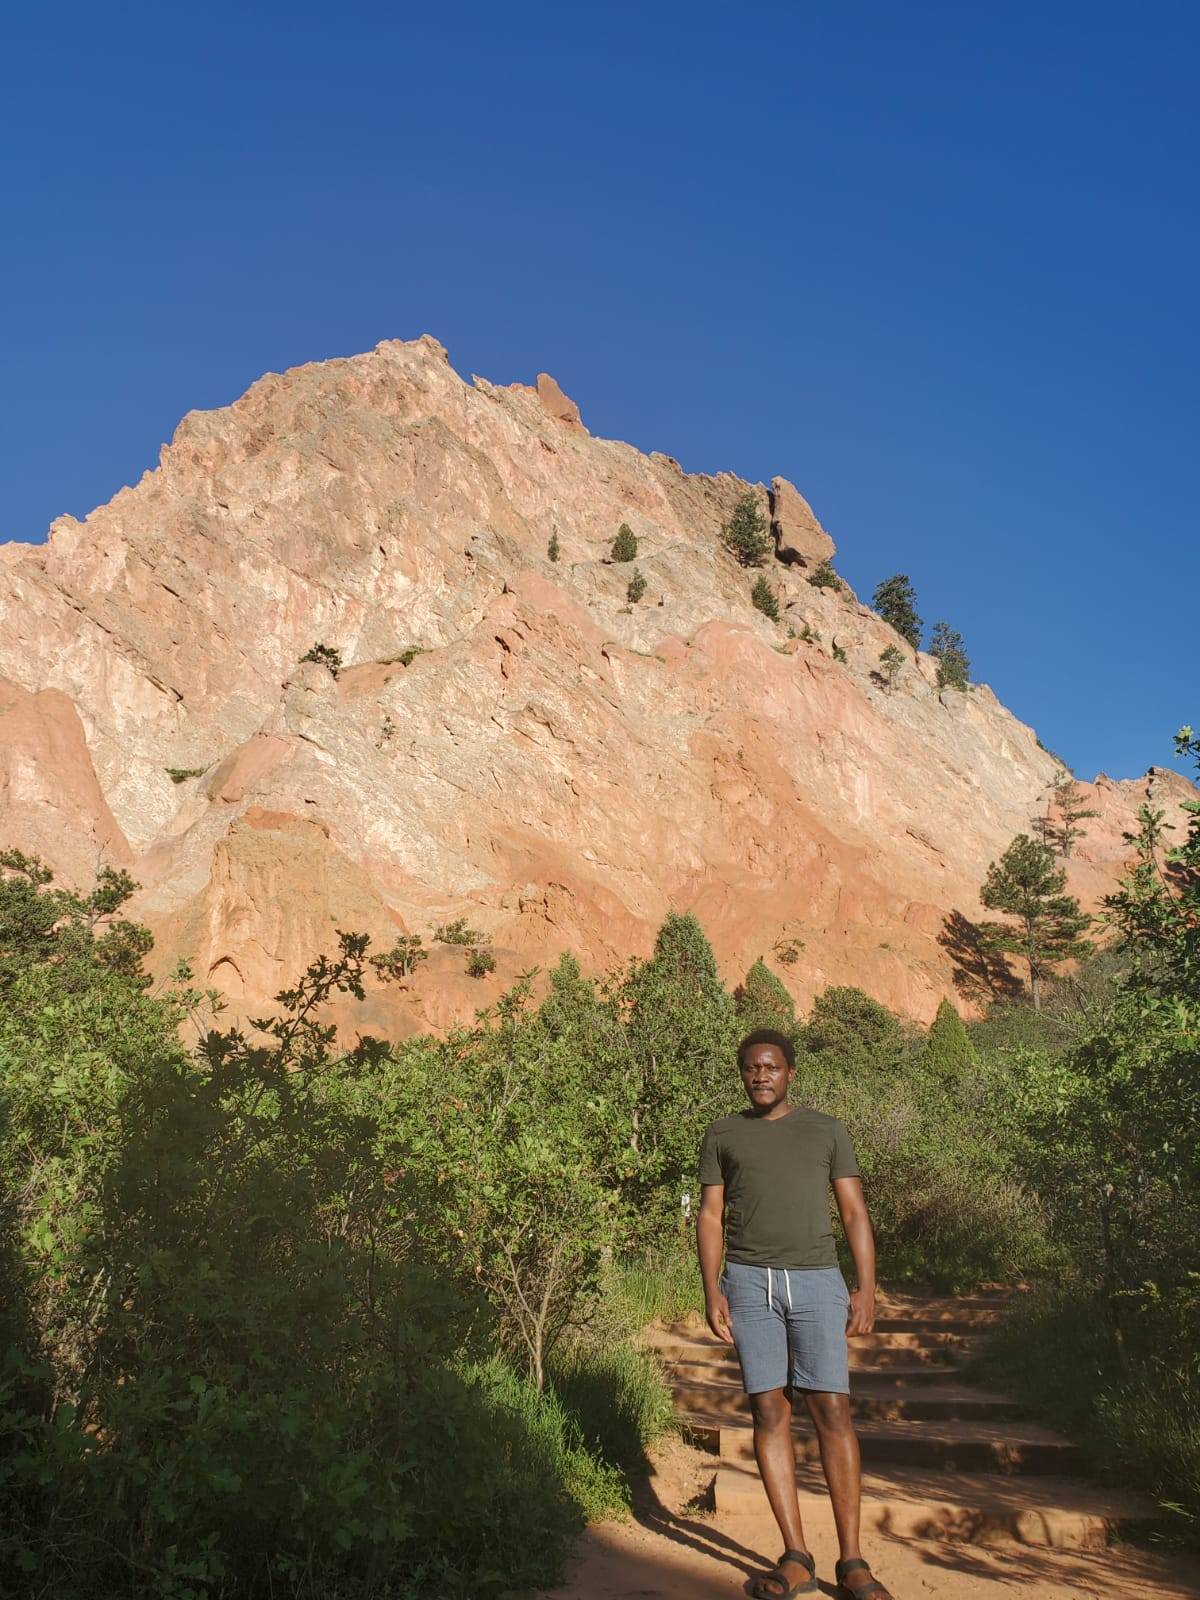
\includegraphics[width=7cm, height=8cm]{TrailWalk}
    \caption{A trail walk in Garden of the Gods, Colorado Springs}
\end{figure}


\subsection*{Section II:  Research Area}
Latency and throughput remain critical performance requirements for internet-based applications in distributed environments such as the cloud-based architecture. Though there have been significant research  done on load balancing in cloud computing environments, a bulk of the research have focused primarily on implementing elasticity in the computing environment by scaling-up(vertical scalability) or  scaling-out(horizontal scalability) \cite{raghava2014comparative,velde2017advanced}. However, a crucial aspect of performance in any cloud architecture is cost of performance as the infrastructure is scaled. MBal\cite{cheng2015memory,hong2013understanding,chavan2014clustered} provides a fundamental approach on orchestrating in-memory technique that presents benefits of cost reduction to cloud users.

MBal proposes two objective functions based on Integer Linear Programming(ILP). The goal of the first function, presented below,  minimizes count of migration operations with a fixed source worker.\\

minimize  
\begin{eqnarray}
    \sum_{i}\sum_{j}X_{ij}^{k} \\
s.t. \    L_{*a} +  \sum_{i}\sum_{j}X_{ia}^{k}L_{i}^{k} -   \sum_{i}\sum_{j}X_{ia}^{k}L_{a}^{k} \leq T_{a}\\
\forall i \in S \backslash a: L_{*i}+\sum_{k}X_{ia}^{k}L_{i}^{k} - \sum_{k}X_{ia}^{k}L_{i}^{k}\leq T_{i}
\end{eqnarray}


where a is the index of the fixed source worker thread; $X_{ij}^{k}$ is 1 if the cachetlet k is migrated from worker i to worker j, 0 otherwise; $ T_{j} $ is the maximum permissible load on worker j; $ L_{*j} $ is the total load on worker j. 

The below git repos has relevance to my research even though it is rudimentary. It provides a read/write memory function based on process id. It can be found at \url{https://github.com/voyula/read-write-memory/blob/master/src/read-write-memory.cpp}


\clearpage
\nocite{*}
\printbibliography

\subsection{The First Section}

I have registered for this course as a prerequisite for a Ph.D. program. Through this course, I hope to learn how to write a research paper in a scientific way.  I hope to understand how to select relevant articles related to my area of research. So, I can improve my practice and knowledge of the latest updates and new topics of my work. I hope to know the correct ways to read research papers, compare between them, present a discussion of those papers. I would be interested to learn how to present my research work and how to write the paper scientifically. In addition, I hope I can recognize the different sections of scientific documents, such as the introduction, methodology,  results and discussion, and conclusion.  I want to learn how to present the contribution of my work easily and clearly. Expectedly, I will learn how to layout my experiment methodology, how to get the result, and how to analyze them. I hope to gain and be able to conduct a comprehensive survey on my field of interest and to write a good paper using scientific techniques, essential and effective statistical methods. Hopefully, I will be able to publish this paper in a good conference or journal. 

\begin{center}

\includegraphics[scale=0.2]{Khalid.jpeg}
\end{center}


 \subsubsection{Git Repo}
I have found code on Github about my research topic Face Recognition using Open-CV \url{https://github.com/Mjrovai/OpenCV-Face-Recognition} which is useful in learning more about face recognition using deep learning.


\subsubsection{Questions and Answer} 
\begin{enumerate}
	\item RR: Very interesting Git repo, I did not know OpenCV included a facial recognition classifier. Do you have much experience with OpenCV?
        \item Answer: I'm new in this area and I'm planning to run multiple classifiers from OpenCV which is a library designed for video and image processing. 

\end{enumerate}

\include{kormene}

\section{Example of Easy Tables}
\csvautotabular{test.csv}


\section*{Better formated Tables}
    \begin{tabular}{r|r|r}%
    % specify table head
    \bf Time (s) & \bf Rel. time (s)& \bf Y Pos
% use head of csv as column names
    \csvreader{test.csv}{}
% specify selected coloumns here
    {\\\hline\csvcoli&\csvcolii&\csvcolvi}
    \end{tabular}
    \clearpage


\end{document}
